%-------------------------------------------------
\documentclass[ks,hauptseminar]{daposterifn}
%-------------------------------------------------
%* options:
%* tnt, hf, tk, mns /default: -none-
%* diplom, master   /default: diplom
%* extern

%%% LANGUAGE %%%
\usepackage[T1]{fontenc}      % correct german hyphenation of word with umlaute
\usepackage{babel}
%\usepackage[latin1]{inputenc} % direct use of german umlaute, utf8 encoding

%%% LAYOUT %%%
%\usepackage[a4paper,top=25mm,left=20mm,right=20mm,bottom=20mm]{geometry} %modify page geometry
%\pagestyle{plain}             % layout with plain page number
\parindent 0pt                % no paragraph indentation

%%% GRAPHICS %%%
\usepackage{graphicx}  % graphical elements
\usepackage{pstricks}  % postscript drawings
\usepackage{textcomp}  % additional symbols
\usepackage{xcolor}    % colored elements, extended package
\usepackage{pgfplots}
\usepackage{tikz}

%%% MATH & SCIENCE %%%
\usepackage{amsmath}   % math formulae
\usepackage{amssymb}   % math symbols
\usepackage{amsfonts}  % additional math fonts
\usepackage{units}     % setting units typographically correct

%%% CODES %%%
\usepackage{verbatim}  % verbatim display/commenting pieces of LaTeX code
\usepackage{listings}  % display of source code listings

%%% BIBLIO %%%
\usepackage[backend=biber,style=numeric]{biblatex}
\usepackage[babel,german=quotes]{csquotes}
\bibliography{literatur.bib}

%%% MISC %%%
\usepackage{pdfpages}  % include pdfs
\usepackage{caption}
\usepackage{subfig}
\usepackage{float}
%\usepackage{morefloats}

\usepackage{hyperref}  % document navigation with hyperlinks (load last)



% % % % % % % % % % % % % %
% % % % %  SETUPS % % % % %
% % % % % % % % % % % % % %
\pgfplotsset{compat=newest}
\pgfplotsset{plot coordinates/math parser=false}

\usetikzlibrary{shapes, arrows, circuits, trees}

\hypersetup{
	%bookmarks=false,            % show bookmarks bar?
	%unicode=false,              % non-Latin characters in Acrobat's bookmarks
	pdftoolbar=true,            % show Acrobat's toolbar?
	pdfmenubar=true,            % show Acrobat's menu?
	pdffitwindow=false,         % window fit to page when opened
	pdfstartview={FitH},        % fits the width of the page to the window
	pdftitle={},      % title
	pdfauthor={Karl-Ludwig Besser},     % author
	pdfsubject={},% subject of the document
	pdfcreator={Karl-Ludwig Besser}               % creator of the document
	pdfproducer={Karl-Ludwig Besser},             % producer of the document
	pdfkeywords={},             % list of keywords
	pdfnewwindow=true,          % links in new window
	colorlinks=true,            % false: boxed links; true: colored links
	linkcolor=black,            % color of internal links
	citecolor=black,            % color of links to bibliography
	filecolor=red,              % color of file links
	urlcolor=blue,              % color of external links
	breaklinks=true             % break urls
}

\lstloadlanguages{matlab}
\lstset{
	%    language=[ANSI]c        % language of code
	%    defaultdialect=ANSI  % default dialect of language
	%    language=    % language of code
	%    language=        % language of code
	basicstyle=\footnotesize,          % fontsize for code
	keywordstyle=\ttfamily\bfseries,   % fontstyle for keywords
	stringstyle=\ttfamily\color{blue}, % fontstyle for non-keywords and strings
	commentstyle=\itshape,             % fontstyle for comments
	extendedchars=true,                % extended (national) characters
	numbers=left,                      % where to put line-numbers
	numberstyle=\tiny,                 % fontsize for line-numbers
	numbersep=10pt,                    % space between numbers and code
	stepnumber=2,                      % step between numbers
	showspaces=false,                  % underline spaces within code
	showstringspaces=false,            % underline spaces within strings
	showtabs=false,                    % underline tabs within strings
	tabsize=2,                         % default tab-size in spaces
	frame=single,                   % frame around code
	backgroundcolor=\color{bgcol},     % background color (needs color package)
	rulesepcolor=\color{shcol},        % shadow color (needs color package)
	captionpos=b,                      % caption-position (bottom)
	breaklines=true,                   % automatic line breaking
	breakatwhitespace=false,           % automatic breaks at whitespace
	breakindent=20pt,                  % indentation of broken lines
	breakautoindent=true,              % automatic indentation of broken lines
	morecomment=[l]{//}                % comments in italics (language dependent)
}


% % % % % % % % % % % % % %
% % % % %  COLORS % % % % %
% % % % % % % % % % % % % %
\definecolor{shcol}{gray}{0.80}
%\definecolor{bgcol}{rgb}{0.99, 0.99, 0.85}
\definecolor{bgcol}{rgb}{1, 1, 1}


% % % % % % % % % % % % % % %
% % % % %  COMMANDS % % % % %
% % % % % % % % % % % % % % %
\newcommand{\dif}{\mathrm{d}}

\tikzset{%
	block/.style    = {draw, thick, rectangle, minimum height = 2em, minimum width = 2em},
	ring/.style     = {draw, thick, circle, minimum size = 2em},
	elipse/.style   = {draw, thick, ellipse, minimum height = 1em},
	sum/.style      = {draw, circle, node distance = 1cm}, % Adder
	input/.style    = {coordinate}, % Input
	output/.style   = {coordinate} % Output
}

% Defining string as labels of certain blocks.
\newcommand{\suma}{\Large$+$}
\newcommand{\inte}{$\displaystyle \int$}
\newcommand{\derv}{\huge$\frac{d}{dt}$}


%-------------------------------------------------
% BITTE HIER PARAMETER SETZEN!
%-------------------------------------------------

\setDAParameter[\LARGE]{Thema}{Synthese von Sprachsignalen}
\setDAParameter{Student}{Karl-Ludwig Besser, Zhongjiu Li, Franz-Marcus Sch\"uffny, Peter Steiner}
\setDAParameter{BetreuerTUD}{PD Dr.-Ing. Ulrich Kordon~\\ Dipl.-Ing. Steffen K\"urbis}
%\setDAParameter{BetreuerExternName}{}
%\setDAParameter{BetreuerExternFirma}{}
\setDAParameter{Hochschullehrer}{Jun.-Prof. Dr.-Ing. Peter Birkholz}
\setDAParameter{VerteidigungDatum}{14.07.2015}

%-------------------------------------------------

%\setStudentPassbild[5.0cm]{./figures/passbild}
%\setStudentWerdegang[\small][1.0ex]{%
%	07/2003\newline
%	Schulabschluss in Sowieso-Dingskirchen
	
%	seit 10/2003\newline
%	Studium Elektrotechnik an der TU Bergakademie Freiberg
	
%	seit 10/2005\newline
%	Studium Elektrotechnik, Studienrichtung Informationstechnik, an der TU Dresden
	
%	10/2007 - 03/2008\newline
%	Auslandsstudium an der �cole Polytechnique F�d�rale de Lausanne, Schweiz
	
%	10/2008 - 03/2009\newline
%	Fachpraktikum bei Firma-Fiktiv und Partner in GanzWoAnders-Blahausen
%}


%-------------------------------------------------
% BEGINN DES DOKUMENTS
%-------------------------------------------------

\begin{document}


\includeDADetails


%* uncomment next line to switch the document language (for caption labels etc.) to English (default: German)
%\selectlanguage{english}


\begin{multicols}{3}


%-------------------------------------------------
% BITTE HIER EIGENEN INHALT EINF�GEN!
%-------------------------------------------------

%-------------------------------------------------
\section*{Einleitung}
%-------------------------------------------------

Im Hauptseminars Kommunikationssysteme wurde das Thema \enquote{Synthese von Sprachsignalen} bearbeitet. Der Fokus lag auf der Erzeugung von Sprachsignalen mittels Formantsynthese. Diese wurde in einem Computerprogramm durch ein Quelle-Filter-Modell realisiert.
Zur Parameterbestimmung war eine vorherige Analyse realer Sprache notwendig.

Mit dieser Thematik besch\"aftigten sich Forscher schon seit mehreren Jahrhunderten.

\begin{figure}[H]
	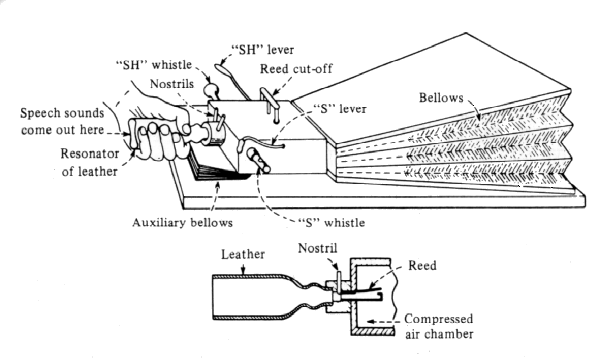
\includegraphics[width = .25\textwidth]{figures/Einleitung/kratzenstein.png}
	\caption{Kratzensteins Resonator, Quelle: }
	\label{fig:kratzenstein}
\end{figure}
--> Hier eine Grafik einf\"ugen - wie macht und zitiert man das richtig? <--

Weitere Meilensteine waren die Entwicklung elektronischer Filter sowie der Einsatz moderner Computertechnik. 

Heutzutage kommen Systeme zur Sprachsynthese zum Beispiel in Navigationsger\"aten und Smartphones zum Einsatz.

%-------------------------------------------------
\section*{Quelle-Filter-Modell}
%-------------------------------------------------

Das Quelle-Filter-Modell versucht eine Zerlegung von Sprachsignalen in Anregungssignale und Filterstrukturen. Durch geeignete Wahl der Modellparameter soll eine m\"oglichst gute Modellierung des menschlichen Artikulationstrakts erreicht werden. 

Die Struktur des Modells, wie es hier verwendet wird, ist in Abbildung \ref{fig:QFM} gezeigt.

\begin{figure}[H]
	\centering
	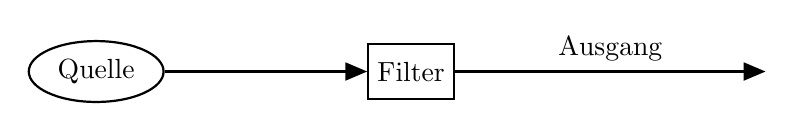
\begin{tikzpicture}[auto, thick, node distance=2cm, >=triangle 45]
\draw
% Block setzen
node at (-1,0)[elipse](input) {Quelle} 
node at (3,0)[block] (filter) {Filter};
% Block verbinden
\draw[->](input) -- node {}(filter);
\draw[->](filter) -- node {Ausgang}(7.5,0);

\end{tikzpicture}
	\caption{Verwendetes Quelle-Filter-Modell}
	\label{fig:QFM}
\end{figure}


%-------------------------------------------------
\section*{Analyse}

Zur Parametrisierung des in \ref{fig:QFM} dargestellten Modells m\"ussen reale Sprachsignale analysiert werden.

Der Schwerpunkt liegt hierbei auf der Bestimmung der Filterparameter. Es werden prim\"ar Bandpassfilter 2. Ordnung eingesetzt. Die drei charakteristischen Parameter sind Mittenfrequenz, Bandbreite und Grundverst\"arkung.

Die Mittenfrequenz wird als Formantfrequenz. Um diese zu bestimmen, wurden verschiedene Analysemethoden verwendet. Von der Software Praat wurde der fertig implementierte Burg-Algorithmus bereitgestellt, selbst nachprogrammiert wurde der Cepstrum-Algorithmus. Au{\ss}erdem wurden die Formantfrequenzen manuell aus dem Spektrum abgelesen, wie in Abbildung \ref{fig:spektrum} dargestellt.

Die 

\begin{figure}
%	\input{as\"olkdjfa\"oskldjfa\"oskljdfa\"oskljdf}
	\caption{Spektrum des Vokals ...}
	\label{fig:spektrum}
\end{figure}
Lorem ipsum dolor sit amet, consectetuer adipiscing elit, sed diam nonummy nibh euismod tincidunt ut laoreet dolore magna aliquam erat volutpat. Ut wisi enim ad minim veniam $c = \sqrt{a^2 + b^2}$, quis nostrud exerci tation ullamcorper suscipit lobortis nisl ut aliquip ex ea commodo consequat.
\begin{alignat*}{1}
	y = \sum_{i=1}^{M} \left[ c_i \, \frac{x_i - \alpha}{1 + \prod_{j=1}^{M} r_{i,j} x_i} + \max \{ \theta_i, \sigma^2 \} \right]
\end{alignat*}
Lorem ipsum dolor sit amet, consectetuer adipiscing elit, sed diam nonummy nibh euismod tincidunt ut laoreet dolore magna aliquam erat volutpat.

Ut wisi enim ad minim veniam, quis nostrud exerci tation ullamcorper suscipit lobortis nisl ut aliquip ex ea commodo consequat.


%-------------------------------------------------
\subsubsection*{Unter\"uberschrift Ebene 3}

\blindtext[1]


%-------------------------------------------------
\subsubsection*{Unter\"uberschrift Ebene 3}

Lorem ipsum dolor sit amet, consectetuer adipiscing elit, sed diam nonummy nibh euismod tincidunt ut laoreet dolore magna aliquam erat volutpat.

\begin{itemize}
	\item Ut ornare est ac arcu molestie sed porttitor.
	\item Aliquam ultricies sollicitudin quam.
	\item Nunc porta placerat arcu, ac bibendum massa adipiscing id. Nulla facilisi.
				Vivamus a arcu ut urna vehicula rhoncus quis vel lectus.
	\item Nullam ornare, sem dictum mollis dictum, ante nulla sollicitudin nunc, in dictum mauris tellus nec dolor. 
\end{itemize}

Ut wisi enim ad minim veniam, quis nostrud exerci tation ullamcorper suscipit lobortis nisl ut aliquip ex ea commodo consequat.

\begin{center}
	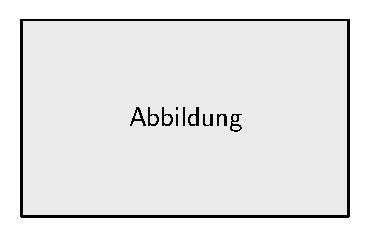
\includegraphics[width=\linewidth]{./figures/abbildung}
	\captionof{figure}{Unterschrift f\"ur Abbildung.\label{fig:abbildung}}
\end{center}

Lorem ipsum dolor sit amet, consectetuer adipiscing elit, sed diam nonummy nibh euismod tincidunt ut laoreet dolore magna aliquam erat volutpat. Ut wisi enim ad minim veniam, quis nostrud exerci tation ullamcorper suscipit lobortis nisl ut aliquip ex ea commodo consequat.

\begin{center}
	\begin{tabularx}{\linewidth}{|l|X|X|}
	  \hline
		jdffdslf & fjdsf jhg lkjgljfdlg jfdj jrgjfdkgeag & jfdfjwgr igjirejg \\ \hline
		ejperg   & jgjk rpe jbhpets jpgfg                & gkfdl gh jthjp trhks tpsjrst\"aj trjs js irithjmn \\ \hline
	\end{tabularx}
	\captionof{table}{Unterschrift f\"ur Tabelle.\label{tab:tabelle}}
\end{center}


%-------------------------------------------------
\subsection*{Unter\"uberschrift Ebene 2}

Donec fringilla rhoncus dolor et pretium. Donec non neque eget mi imperdiet porttitor. Nulla facilisi. Ut porta justo nec tortor sollicitudin in elementum sem lobortis. Sed non cursus nunc. Morbi ac felis mollis dolor pulvinar ullamcorper id nec dui. Sed id nibh magna, sit amet laoreet elit.
\begin{enumerate}
	\item Duis adipiscing venenatis risus, et condimentum risus commodo nec.
	\item Quisque ut leo quis leo porta pellentesque ut sit amet leo. Phasellus quis pharetra nisl.
	\item Fusce imperdiet rhoncus ante, sed iaculis elit euismod vel.
\end{enumerate}
Aenean ac nulla ipsum. Sed nulla dui, consectetur sit amet ultrices eget, semper nec ipsum. Pellentesque lacinia ornare sapien, ac accumsan nulla congue eget. Aliquam gravida nulla id justo egestas accumsan.

Vestibulum convallis malesuada faucibus. Vestibulum ligula turpis, venenatis vel gravida at, eleifend eget tortor. Phasellus blandit nisi vel leo euismod a vestibulum est vestibulum. Duis convallis dignissim turpis. Nam ullamcorper molestie urna et iaculis.


%-------------------------------------------------
\section*{Zusammenfassung}
%-------------------------------------------------

Aenean ac nulla ipsum. Sed nulla dui, consectetur sit amet ultrices eget, semper nec ipsum. Pellentesque lacinia ornare sapien, ac accumsan nulla congue eget. Aliquam gravida nulla id justo egestas accumsan.
Vestibulum convallis malesuada faucibus. Vestibulum ligula turpis, venenatis vel gravida at, eleifend eget tortor. Phasellus blandit nisi vel leo euismod a vestibulum est vestibulum. Duis convallis dignissim turpis. Nam ullamcorper molestie urna et iaculis.

\blindtext[1]

\blindtext[1]


\end{multicols}


\end{document}